% Font options: 10pm, 11pt, 12pt
% Align headings left instead of center: nocenter
\documentclass[xcolor=x11names,compress]{beamer}\usepackage[]{graphicx}\usepackage[]{color}
% maxwidth is the original width if it is less than linewidth
% otherwise use linewidth (to make sure the graphics do not exceed the margin)
\makeatletter
\def\maxwidth{ %
  \ifdim\Gin@nat@width>\linewidth
    \linewidth
  \else
    \Gin@nat@width
  \fi
}
\makeatother

\definecolor{fgcolor}{rgb}{0.345, 0.345, 0.345}
\newcommand{\hlnum}[1]{\textcolor[rgb]{0.686,0.059,0.569}{#1}}%
\newcommand{\hlstr}[1]{\textcolor[rgb]{0.192,0.494,0.8}{#1}}%
\newcommand{\hlcom}[1]{\textcolor[rgb]{0.678,0.584,0.686}{\textit{#1}}}%
\newcommand{\hlopt}[1]{\textcolor[rgb]{0,0,0}{#1}}%
\newcommand{\hlstd}[1]{\textcolor[rgb]{0.345,0.345,0.345}{#1}}%
\newcommand{\hlkwa}[1]{\textcolor[rgb]{0.161,0.373,0.58}{\textbf{#1}}}%
\newcommand{\hlkwb}[1]{\textcolor[rgb]{0.69,0.353,0.396}{#1}}%
\newcommand{\hlkwc}[1]{\textcolor[rgb]{0.333,0.667,0.333}{#1}}%
\newcommand{\hlkwd}[1]{\textcolor[rgb]{0.737,0.353,0.396}{\textbf{#1}}}%
\let\hlipl\hlkwb

\usepackage{framed}
\makeatletter
\newenvironment{kframe}{%
 \def\at@end@of@kframe{}%
 \ifinner\ifhmode%
  \def\at@end@of@kframe{\end{minipage}}%
  \begin{minipage}{\columnwidth}%
 \fi\fi%
 \def\FrameCommand##1{\hskip\@totalleftmargin \hskip-\fboxsep
 \colorbox{shadecolor}{##1}\hskip-\fboxsep
     % There is no \\@totalrightmargin, so:
     \hskip-\linewidth \hskip-\@totalleftmargin \hskip\columnwidth}%
 \MakeFramed {\advance\hsize-\width
   \@totalleftmargin\z@ \linewidth\hsize
   \@setminipage}}%
 {\par\unskip\endMakeFramed%
 \at@end@of@kframe}
\makeatother

\definecolor{shadecolor}{rgb}{.97, .97, .97}
\definecolor{messagecolor}{rgb}{0, 0, 0}
\definecolor{warningcolor}{rgb}{1, 0, 1}
\definecolor{errorcolor}{rgb}{1, 0, 0}
\newenvironment{knitrout}{}{} % an empty environment to be redefined in TeX

\usepackage{alltt}
%\documentclass[xcolor=x11names,compress,handout]{beamer}
\usepackage[]{graphicx}
\usepackage[]{color}
\usepackage{booktabs}
\usepackage{hyperref}
\usepackage{tikz}
\usepackage{multirow}
\usepackage{multicol}
\usepackage{dcolumn}
\usepackage{bigstrut}
\usepackage{amsmath} 
\usepackage{colortbl}
\usepackage{amssymb}
%\newcommand{\done}{\cellcolor{teal}#1}

%% Beamer Layout %%%%%%%%%%%%%%%%%%%%%%%%%%%%%%%%%%
\useoutertheme[subsection=false,shadow]{miniframes}
\useinnertheme{default}
\usefonttheme{serif}
\usepackage{Arev}
\usepackage{pdfpages}

\setbeamerfont{title like}{shape=\scshape}
\setbeamerfont{frametitle}{shape=\scshape, size=\normalsize}

\definecolor{dkblue}{RGB}{0,0,102}

\setbeamercolor*{lower separation line head}{bg=dkblue} 
\setbeamercolor*{normal text}{fg=black,bg=white} 
\setbeamercolor*{alerted text}{fg=red} 
\setbeamercolor*{example text}{fg=black} 
\setbeamercolor*{structure}{fg=black} 
 
\setbeamercolor*{palette tertiary}{fg=black,bg=black!10} 
\setbeamercolor*{palette quaternary}{fg=black,bg=black!10} 

\renewcommand{\(}{\begin{columns}}
\renewcommand{\)}{\end{columns}}
\newcommand{\<}[1]{\begin{column}{#1}}
\renewcommand{\>}{\end{column}}

\newcolumntype{L}{>{\centering\arraybackslash}m{.8cm}}

\setbeamertemplate{navigation symbols}{} 
\setbeamertemplate{footline}[frame number]
\setbeamertemplate{caption}{\raggedright\insertcaption\par}

\setbeamersize{text margin left=5pt,text margin right=5pt}

\AtBeginSection{\frame{\sectionpage}}
\hypersetup{
    colorlinks,
    linkcolor={red!50!black},
    citecolor={blue!50!black},
    urlcolor={blue!80!black}
}

\setbeamercolor{block title}{use=structure,fg=white,bg=structure.fg!75!orange}
\setbeamercolor{block body}{parent=normal text,use=block title,bg=block title.bg!10!bg}

%%%%%%%%%%%%%%%%%%%%%%%%%%%%%%%%%%%%%%%%%%%%%%%%%%



\title{FLS 6441 - Methods III: Explanation and Causation}
\subtitle{Week 6 - Instrumental Variables}
\author{Jonathan Phillips}
\date{April 2020}
\IfFileExists{upquote.sty}{\usepackage{upquote}}{}
\begin{document}  

\frame{\titlepage}

\section{Instrumental Variables}

\begin{frame}
\frametitle{Instrumental Variables}
\begin{itemize}
\item What can we do when the treatment assignment mechanism is not 'as-if' random?
\pause
\begin{itemize}
\item Eg. An omitted variable affects both treatment and the outcome
\end{itemize}
\pause
\item Natural experiments focus on a specific \textbf{component} of treatment assignment that is 'as-if' random
\pause
\item An 'instrument' is a variable which assigns treatment in an 'as-if' random way
\pause
\begin{itemize}
\item I.e. Independent of potential outcomes
\pause
\item Even if other variables linked to potential outcomes \textbf{also} affect treatment
\end{itemize}
\end{itemize}
\end{frame}

\begin{frame}
\frametitle{Instrumental Variables}
\begin{knitrout}
\definecolor{shadecolor}{rgb}{0.969, 0.969, 0.969}\color{fgcolor}
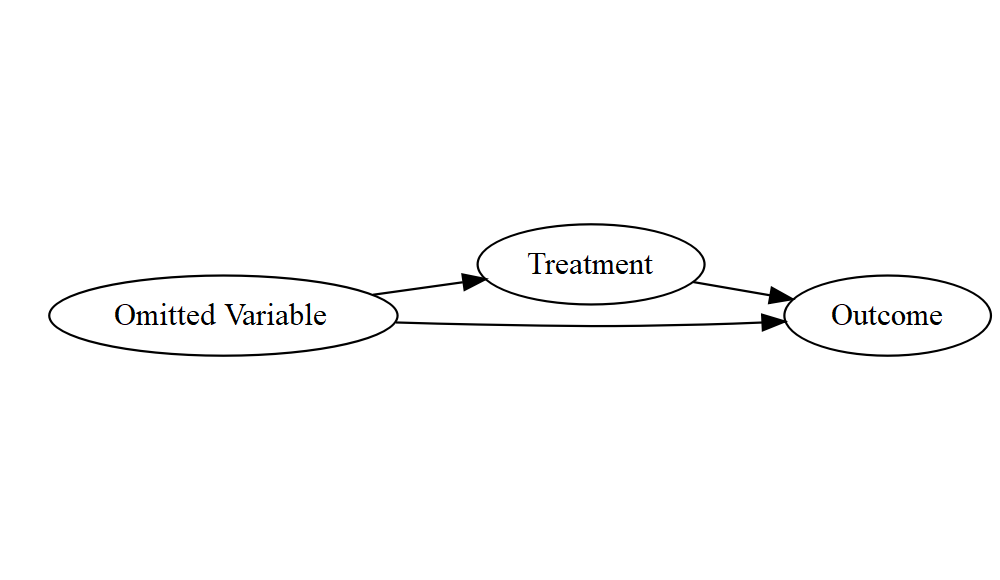
\includegraphics[width=\maxwidth]{figure/dag1-1} 

\end{knitrout}
\end{frame}

\begin{frame}
\frametitle{Instrumental Variables}
\begin{knitrout}
\definecolor{shadecolor}{rgb}{0.969, 0.969, 0.969}\color{fgcolor}
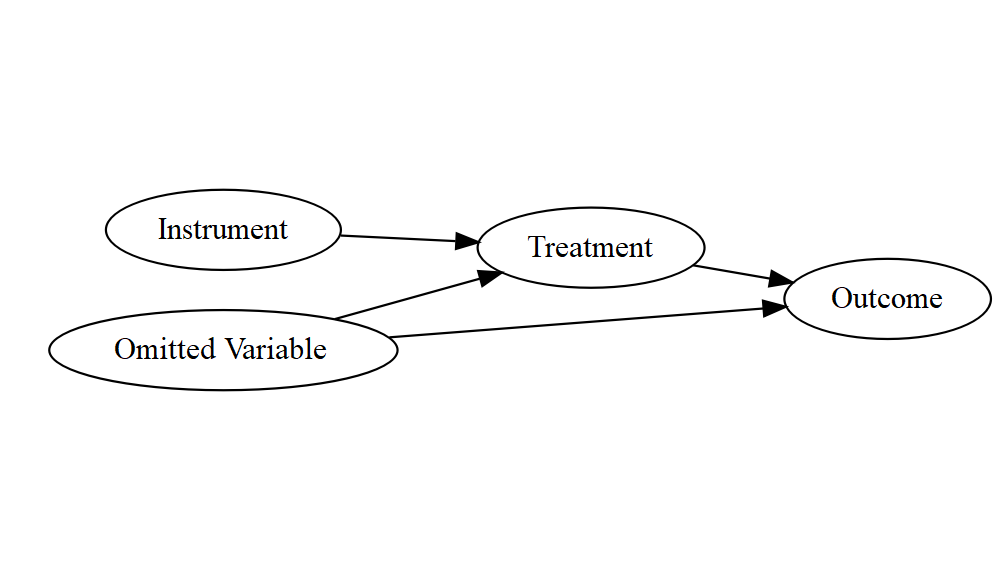
\includegraphics[width=\maxwidth]{figure/dag2-1} 

\end{knitrout}
\end{frame}

\begin{frame}
\frametitle{Instrumental Variables}
\begin{knitrout}
\definecolor{shadecolor}{rgb}{0.969, 0.969, 0.969}\color{fgcolor}
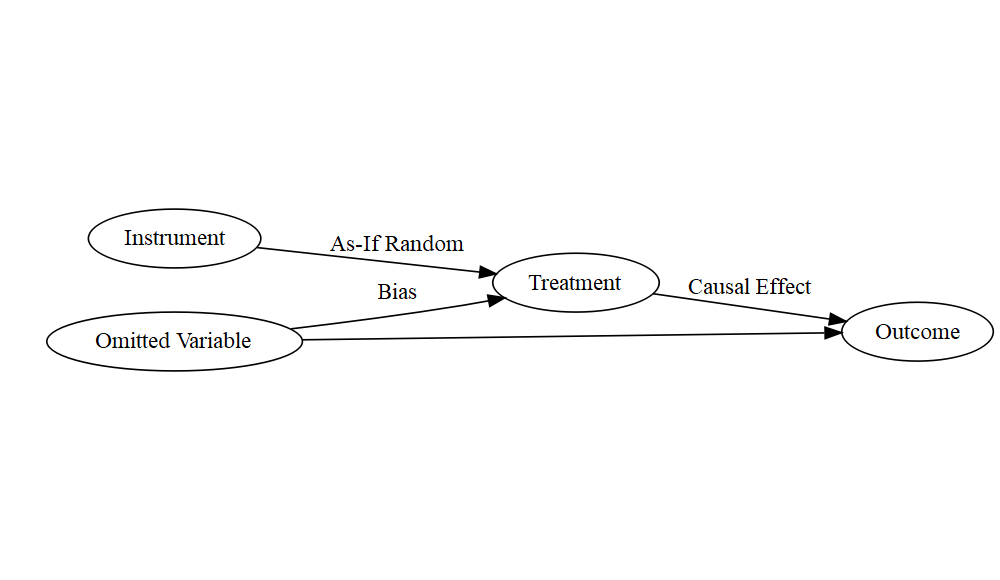
\includegraphics[width=\maxwidth]{figure/dag3-1} 

\end{knitrout}
\end{frame}

\begin{frame}
\frametitle{Instrumental Variables}
\begin{knitrout}
\definecolor{shadecolor}{rgb}{0.969, 0.969, 0.969}\color{fgcolor}
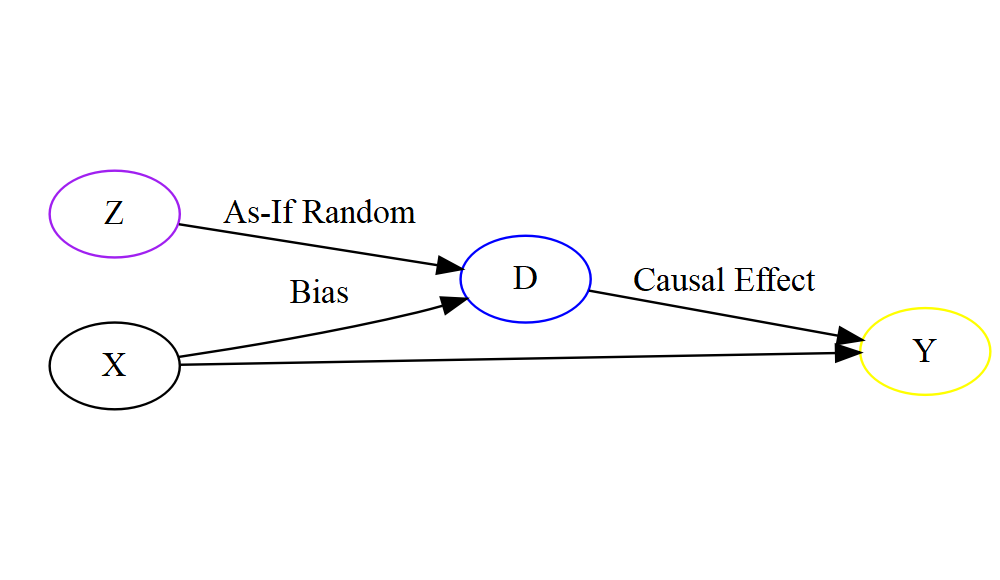
\includegraphics[width=\maxwidth]{figure/dag4-1} 

\end{knitrout}
\end{frame}


\begin{frame}
\frametitle{Instrumental Variables}
\begin{itemize}
\item Example Instruments:
\begin{itemize}
\item Rainfall for conflict 
\item Gender of first two children for effect of having a third child
\item Distance from the coast for exposure to slave trade
\end{itemize}
\end{itemize}
\end{frame}

\begin{frame}
\frametitle{Instrumental Variables Assumption}
\begin{multicols}{2}
\begin{itemize}
\item 1. \textbf{Strong 'First Stage':}
\pause
\item Instrument Predicts Treatment
\pause
\item We can assess this with a simple regression:
\pause
\item $\textcolor{blue}{D_i} = \alpha + \beta \textcolor{purple}{Z_i} + \epsilon_i$
\pause
\item The instrument should be a significant predictor of treatment
\pause
\item Rule-of-thumb: $F-statistic > 10$
\end{itemize}
\columnbreak
\begin{itemize}
\item 2. \textbf{Exclusion Restriction} 
\pause
\item The Instrument \textit{ONLY} affects the outcome through its effect on treatment, and not directly
\pause
\item Formally, $cov(\textcolor{purple}{Z_i}, \epsilon_i \text{ in } \textcolor{yellow}{Y_i} \sim \textcolor{blue}{D_i})=0$
\pause
\item \textbf{We cannot test or prove this assumption!}
\pause
\item Theory and qualitative evidence needed
\end{itemize}
\end{multicols}
\end{frame}

\begin{frame}
\frametitle{Instrumental Variables Methodologies}
\begin{multicols}{2}
\begin{itemize}
\item 1. \textbf{2-Stage Least Squares (2SLS):}
\pause
\item Isolate the variation in treatment caused by the instrument: $\textcolor{blue}{D_i} = \alpha + \beta_1 \textcolor{purple}{Z_i} + \epsilon_i$
\pause
\item Save the predicted values from this regression: $\textcolor{blue}{\hat{D_i}} = \hat{\alpha} + \hat{\beta_1} \textcolor{purple}{Z_i}$
\pause
\item Estimate how the predicted values affect the outcome: $\textcolor{yellow}{Y_i} = \alpha + \beta_2 \textcolor{blue}{\hat{D_i}}$
\pause
\item Interpret the coefficient on $\textcolor{blue}{\hat{D_i}}$
\pause
\item But our Standard Errors won't be accurate
\end{itemize}
\columnbreak
\begin{itemize}
\item 2. \textbf{All-in-one Package} 
\pause
\item Use an all-in-one package, eg. \textit{ivreg} in the \textit{AER} package
\pause
\item Specify the formula: $\textcolor{yellow}{Y_i} \sim \textcolor{blue}{D_i} | \textcolor{purple}{Z_i}$
\pause
\item Interpret the coefficient on $\textcolor{blue}{D_i}$
\end{itemize}
\end{multicols}
\end{frame}

\begin{frame}
\frametitle{Instrumental Variables}
\begin{itemize}
\item Types of IV Regressions:
\pause
\begin{enumerate}
\item \textbf{Biased Regression:} The regression ignoring omitted variable bias: $\textcolor{yellow}{Y_i} \sim \textcolor{blue}{D_i}$
\pause
\item \textbf{First-Stage Regression:} Checking the instrument is valid: $\textcolor{blue}{D_i} \sim \textcolor{purple}{Z_i}$
\pause
\item \textbf{IV Regression:} All-in-one estimate of the effect of treatment on the outcome: $\textcolor{yellow}{Y_i} \sim \textcolor{blue}{D_i} | \textcolor{purple}{Z_i}$
\pause
\item \textbf{2-Stage Least Squares:} Two linear regressions: correct coefficient, wrong p-value: $\textcolor{blue}{D_i} \sim \textcolor{purple}{Z_i}$, then $\textcolor{yellow}{Y_i} \sim \textcolor{blue}{\hat{D_i}}$
\pause
\item \textbf{Reduced-Form Regression:} Estimate of the Instrument on the Outcome, \textit{ignoring treatment}: $\textcolor{yellow}{Y_i} \sim \textcolor{purple}{Z_i}$
\end{enumerate}
\end{itemize}
\end{frame}

\begin{frame}
\frametitle{Example}
\begin{itemize}
\item \textbf{Our research question:} How does \textcolor{blue}{economic growth} affect \textcolor{yellow}{conflict}?
\pause
\item \textbf{Our instrument for treatment:} \textcolor{purple}{Low Rainfall}
\pause
\begin{enumerate}
\item \textbf{First Stage:} \textcolor{purple}{Low Rainfall} -> \textcolor{blue}{-Growth} \pause \checkmark
\pause
\item \textbf{Exclusion Restriction:} \textcolor{purple}{Low Rainfall} \textit{only} affects \textcolor{yellow}{Conflict} through \textcolor{blue}{Economic Growth} \pause ?
\end{enumerate}
\end{itemize}
\end{frame}

\begin{frame}
\frametitle{Example}
\begin{itemize}
\item \textbf{Our research question:} How does \textcolor{blue}{economic growth} affect \textcolor{yellow}{conflict}?
\item \textbf{Our instrument for treatment:} \textcolor{purple}{Low Rainfall}
\item \textbf{First-Stage Regression:} $\textcolor{blue}{Growth_i} = 0.12 - 0.1^{*} \textcolor{purple}{Rainfall_i} + \epsilon_i$
\pause
\item \textbf{Fitted values from First-Stage Regression:} $\textcolor{blue}{\hat{Growth_i}} = 0.12 - 0.1^{*} \textcolor{purple}{0.5} + \epsilon_i$
\end{itemize}
\end{frame}

\begin{frame}
\frametitle{Example}
\begin{itemize}
\item \textbf{Our research question:} How does \textcolor{blue}{economic growth} affect \textcolor{yellow}{conflict}?
\item \textbf{Our instrument for treatment:} \textcolor{purple}{Low Rainfall}
\item \textbf{First-Stage Regression:} $\textcolor{blue}{Growth_i} = 0.12 - 0.1^{*} \textcolor{purple}{Rainfall_i} + \epsilon_i$
\item \textbf{Fitted values from First-Stage Regression:} $\textcolor{blue}{0.07} = 0.12 - 0.1^{*} \textcolor{purple}{0.5}$
\end{itemize}
\end{frame}

\begin{frame}
\frametitle{Example}
\begin{itemize}
\item \textbf{Our research question:} How does \textcolor{blue}{economic growth} affect \textcolor{yellow}{conflict}?
\item \textbf{Our instrument for treatment:} \textcolor{purple}{Low Rainfall}
\item \textbf{First-Stage Regression:} $\textcolor{blue}{Growth_i} = 0.12 - 0.1^{*} \textcolor{purple}{Rainfall_i} + \epsilon_i$
\item \textbf{Fitted values from First-Stage Regression:} $\hat{\textcolor{blue}{Growth}} = \textcolor{purple}{0.07, 0.02, 0.06, 0.12, 0.03...}$
\pause
\item \textbf{Second-Stage Regression:} $\textcolor{yellow}{Conflict_i} = \alpha + \beta_2 \textcolor{blue}{\hat{Growth_i}} + \epsilon_i$
\end{itemize}
\end{frame}

\begin{frame}
\frametitle{Example}
\begin{itemize}
\item \textbf{Our research question:} How does \textcolor{blue}{economic growth} affect \textcolor{yellow}{conflict}?
\item \textbf{Our instrument for treatment:} \textcolor{purple}{Low Rainfall}
\item \textbf{First-Stage Regression:} $\textcolor{blue}{Conflict_i} = 0.02 + 0.1^{*} \textcolor{purple}{Rainfall_i} + \epsilon_i$
\item \textbf{Fitted values from First-Stage Regression:} $\textcolor{blue}{\hat{Conflict_i}} = \textcolor{purple}{0.07, 0.02, 0.06, 0.12, 0.03...}$
\item \textbf{Second-Stage Regression:} $\textcolor{yellow}{Conflict_i} = 1.2 - 0.04^{*} \textcolor{blue}{\hat{Growth_i}} + \epsilon_i$
\end{itemize}
\end{frame}

\begin{frame}
\frametitle{LATE}
\begin{itemize}
\item IV \textbf{Interpretation}:
\pause
\begin{itemize}
\item Your coefficient is a causal estimate ONLY for units that were actually treated \textbf{because of the instrument}
\pause
\item They don't tell us about the causal effect for other units that \textit{never responded to the instrument}
\pause
\item Eg. For places where conflict started because of ethnic tensions or an accident
\end{itemize}
\end{itemize}
\pause
\begin{block}{Local Average Treatment Effect (LATE)}
The Average Treatment Effect among the subset of units who are treated because of the instrument: \\
$(\textcolor{blue}{D_i}|\textcolor{purple}{Z_i}=0) = 0$ and $(\textcolor{blue}{D_i}|\textcolor{purple}{Z_i}=1) = 1$
\end{block}
\begin{itemize}
\pause
\item Remember, these 'Local' units might be very rare and unusual so our estimate might be very difficult to generalize
\end{itemize}
\end{frame}

\section{Instrumenting for Institutions}

\begin{frame}
\frametitle{Instrumenting for Institutions}
\begin{itemize}
\item Acemoglu \& Robinson (2001)
\begin{itemize}
\item \textbf{Theory:} Non-electoral \textbf{institutions} (property rights, rule of law, checks and balances) cause economic growth
\pause
\end{itemize}
\item What is the inferential problem here?
\pause
\item Can we run a field experiment?
\pause
\item Can we find a natural experiment?
\end{itemize}
\end{frame}

\begin{frame}
\frametitle{Instrumenting for Institutions}
\begin{itemize}
\item They need an Instrumental Variable that:
\pause
\begin{enumerate}
\item \textbf{First Stage:} \pause Predicts Institutions
\pause
\item \textbf{Exclusion Restriction:} \pause \textit{Only} affects growth through institutions
\end{enumerate}
\pause
\item They make the \textit{argument} that Settler (soldier) mortality rates are an appropriate instrument for institutions
\end{itemize}
\end{frame}


\begin{frame}
\frametitle{Instrumenting for Institutions}
\begin{itemize}
\item \textbf{Population:} \pause Ex-colonies
\pause
\item \textbf{Sample:} \pause Ex-colonies
\pause
\item \textbf{Treatment:} \pause \textcolor{blue}{'Settler' Institutions} in ex-colonies (measured by 'risk of expropriation' index 1985-95)
\pause
\item \textbf{Control:} \pause 'Extractive' institutions
\pause
\item \textbf{Outcome:} \pause \textcolor{yellow}{Growth rates} in 1995
\pause
\item \textbf{Treatment Assignment Mechniams:} \pause Messy! But high settler mortality rates led to extractive institutions
\pause
\item \textbf{Instrument:} \pause \textcolor{purple}{Settler (soldier) mortality rates}
\end{itemize}
\end{frame}

\begin{frame}
\frametitle{Instrumenting for Institutions}
\begin{itemize}
\item \textbf{First Stage:} \pause \textcolor{purple}{Settler mortality rates} predict \textcolor{blue}{institutions}
\pause
\item Supporting Evidence:
\pause
\item ``Mortality rates faced by the settlers more than 100 years ago explains over 25 percent of the variation in current institutions.''
\end{itemize}
\end{frame}

\begin{frame}
\frametitle{Instrumenting for Institutions}
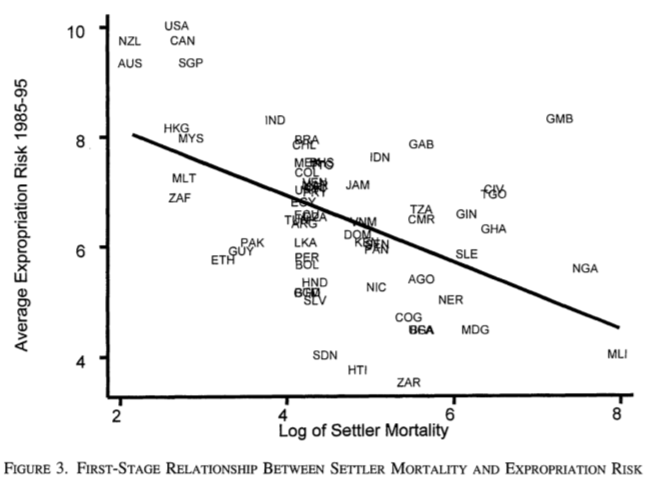
\includegraphics[scale=0.38]{AJR_first_stage.png}
\end{frame}

\begin{frame}
\frametitle{Instrumenting for Institutions}
\begin{itemize}
\item \textbf{Exclusion Restriction:} \pause \textcolor{purple}{Settler mortality rates} ONLY affect \textcolor{yellow}{growth} through \textcolor{blue}{institutions}
\pause
\item Supporting Evidence:
\begin{itemize}
\item \textcolor{purple}{Mortality rates} for locals are low and don't affect human capital or \textcolor{yellow}{growth} directly, due to local immunity
\pause
\item Control for other possible correlated variables - geography, climate, etc.
\end{itemize}
\end{itemize}
\end{frame}

\begin{frame}
\frametitle{Instrumenting for Institutions}
\begin{itemize}
\item Methodology:
\begin{itemize}
\item $\textcolor{blue}{Institutions_i} = \alpha + \beta_0 \textcolor{purple}{Settler\_Mortality_i} + \epsilon_i$
\item $\textcolor{yellow}{Growth_i} = \alpha + \beta_1 \textcolor{blue}{\hat{Institutions_i}} + \epsilon_i$
\end{itemize}
\end{itemize}
\end{frame}

\begin{frame}
\frametitle{Instrumenting for Institutions}
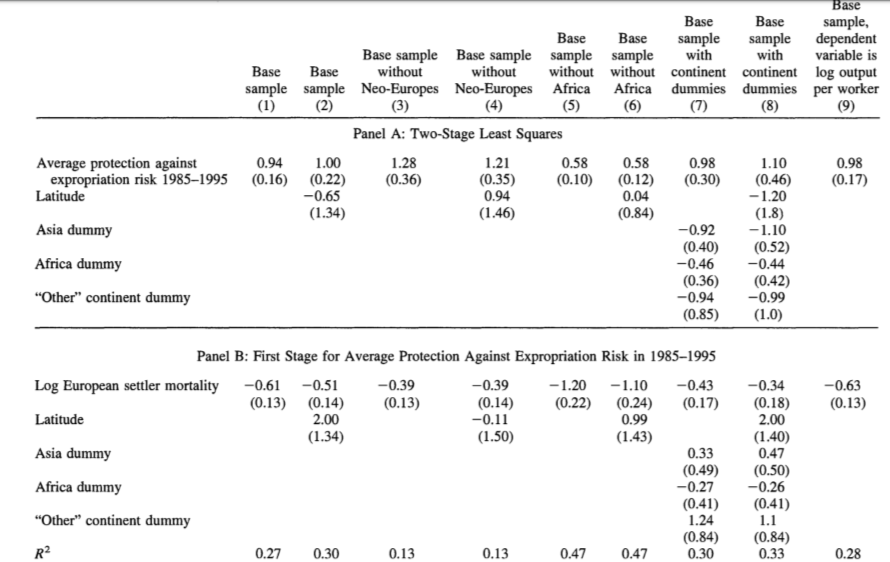
\includegraphics[scale=0.36]{AJR_results.png}
\end{frame}

\begin{frame}
\frametitle{Instrumenting for Institutions}
\begin{itemize}
\item \textbf{Results:} Improving Nigeria's institutions to Chile's level would raise GDP 7-fold
\end{itemize}
\end{frame}

\section{Non-Compliance in Experiments}

\begin{frame}
\frametitle{Non-Compliance in Experiments}
\begin{itemize}
\item Sometimes field experiments don't work perfectly
\pause
\begin{itemize}
\item Eg. We offer free health insurance to families at random, but some reject the offer
\pause
\item Who rejects treatment?
\pause
\item Those that decline treatment are \textit{different} to those that accept (eg. richer)
\pause
\end{itemize}
\item We cannot just compare units that \textit{actually} received treatment to those that did not
\pause
\item Those groups are no longer 'balanced'
\pause
\item Omitted variable bias has returned!
\end{itemize}
\end{frame}

\begin{frame}
\frametitle{Non-Compliance in Experiments}

\begin{knitrout}
\definecolor{shadecolor}{rgb}{0.969, 0.969, 0.969}\color{fgcolor}
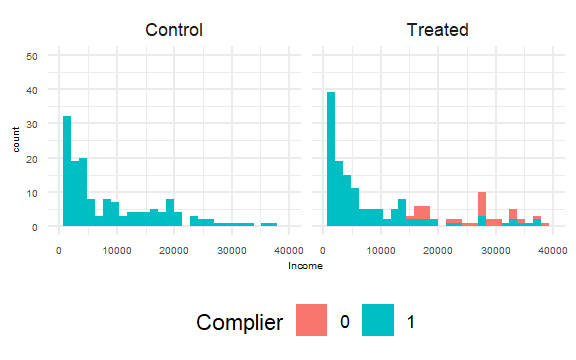
\includegraphics[width=\maxwidth]{figure/unnamed-chunk-1-1} 

\end{knitrout}

\end{frame}

\begin{frame}
\frametitle{Non-Compliance in Experiments}
\begin{itemize}
\item We can divide our units into four types depending on how they accept or reject treatment assignment:
\end{itemize}
\begin{table}[htbp]
  \centering
  \caption{Treatment Status: }
    \begin{tabular}{|p{3cm}|p{3cm}|p{3cm}|}
    \hline
    \multicolumn{1}{|p{3cm}|}{\textbf{If Assigned to Control}} & \multicolumn{1}{p{3cm}|}{\textbf{If Assigned to Treatment}} & \textbf{Unit Type} \bigstrut\\
    \hline
    0     & 1     & Complier \bigstrut\\
    \hline
    0     & 0     & Never-taker \bigstrut\\
    \hline
    1     & 1     & Always-taker \bigstrut\\
    \hline
    1     & 0     & Defier \bigstrut\\
    \hline
    \end{tabular}%
  \label{tab:addlabel}%
\end{table}%
\begin{itemize}
\item Assignment to Treatment is now a separate step prior to treatment - so we can consider it like an instrument, $Z_i$
\end{itemize}
\end{frame}

\begin{frame}
\frametitle{Non-Compliance in Experiments}
\begin{table}[htbp]
  \centering
    \begin{tabular}{c|c|c}
    \multicolumn{1}{p{3cm}}{$D_i(Z_i=0)$} & \multicolumn{1}{p{3cm}}{$D_i(Z_i=1)$} & \multicolumn{1}{l}{} \\
    \hline
    \multicolumn{1}{p{3cm}|}{Treatment Status If Assigned to Control} & \multicolumn{1}{p{3cm}|}{Treatment Status If Assigned to Treatment} & \multicolumn{1}{p{3cm}}{Type?} \\
    \hline
    0     & 1     &  \\
    0     & 0     &  \\
    0     & 1     &  \\
    1     & 0     &  \\
    1     & 1     &  \\
    0     & 0     &  \\
    0     & 1     &  \\
    1     & 0     &  \\
    \end{tabular}%
  \label{tab:addlabel}%
\end{table}%

\end{frame}

\begin{frame}
\frametitle{Non-Compliance in Experiments}
\begin{itemize}
\item Simple difference-in-means estimates of treatment are biased
\pause
\item But we can still use the randomized component of \textbf{treatment assignment as an instrumental variable}
\pause
\end{itemize}
\begin{block}{Local Average Treatment Effect (LATE)}
The Average Treatment Effect \textit{among Compliers}
\end{block}
\begin{itemize}
\item LATE just means we \textit{cannot} learn anything about Never-takers and Always-takers from our Instrumental Variable
\pause
\begin{itemize}
\item Because the instrument \textit{can't} do anything to affect treatment for these units
\end{itemize}
\pause
\item Never-takers and Always-takers are balanced across treatment assignment and do not affect the difference-in-means
\pause
\item We also need to \textbf{assume} Defiers don't exist
\end{itemize}
\end{frame}

\begin{frame}
\frametitle{Non-Compliance in Experiments}
\begin{itemize}
\item Two methodologies for Experiments with Non-Compliance
\end{itemize}
\begin{multicols}{2}
\begin{itemize}
\item \textbf{1. Intention-to-Treat Analysis}
\pause
\item The Effect of Treatment \textbf{Assignment} (the Instrument) on the Outcome
\pause
\item $\textcolor{yellow}{Y_i} ~ \alpha + \beta \textcolor{purple}{Z_i} + \epsilon_i$
\pause
\item A BIASED estimate (<LATE estimate)
\pause
\item For the FULL sample
\end{itemize}
\columnbreak
\begin{itemize}
\item \textbf{2. LATE Instrumental Variables Analysis}
\pause
\item The Effect of Treatment on the Outcome
\pause
\item $\textcolor{yellow}{Y_i} ~ \alpha + \beta \textcolor{blue}{D_i}|\textcolor{purple}{Z_i} + \epsilon_i$
\pause
\item An UNBIASED estimate
\pause
\item Only for COMPLIERS
\end{itemize}
\end{multicols}
\end{frame}

\begin{frame}
\frametitle{Non-Compliance in Experiments}
\begin{itemize}
\item The \textbf{'Strong First-Stage'} assumption here requires that treatment assignment affects treatment for at least some people
\pause
\item The \textbf{'Exclusion Restriction'} assumption requires that outcomes depend on treatment and not treatment assignment
\begin{itemize}
\item So being labelled 'treatment group' (without treatment) doesn't affect your outcome
\end{itemize}
\end{itemize}
\end{frame}


\end{document}
